% ******** Приклад оформлення документа за ДСТУ 3008-95 ********
% ******************** автор: Тавров Д. Ю. *********************

% зазначаємо стильовий файл, який будемо використовувати
\documentclass{udstu}

\addbibresource{refs.bib}

% починаємо верстку документа
\begin{document}

% створимо титульний аркуш
% за допомогою спеціальної команди
% \maketitlepage{params},
% де params --- це розділені комами пари "параметр={значення}"
\maketitlepage{
% StudentName --- прізвище, ініціали студента
	StudentName={Скорденко Д. О.},
% StudentMale --- стать студента (true, якщо чоловік, false --- якщо жінка)
	StudentMale=true,
% StudentGroup --- група студента
	StudentGroup={КМ-01},
% Title --- назва
	Title={Пояснювальна записка до курсового проекту\\ із дисципліни \\ \invcommas{Алгоритми і системи комп'ютерної математики}\\
	на тему \\ \invcommas{Автоматична аннотація зображень за допомогою нейронних мереж}},
% SupervisorDegree --- науковий ступінь, учене звання керівника роботи
% якщо наукового ступеня немає, можна відповідний рядочок пропустити
	SupervisorDegree={асистент кафедри ПМА},
% SupervisorName --- прізвище, ініціали керівника роботи
	SupervisorName={Ковальчик-Химюк Л. О.}
}


% Створюємо анотацію
\abstractUkr

В даній роботі описано мультимодальну систему маркування зображень, в якій зроблено акцент на трьох апспектах:
висока точність, використання тексту в якості додаткової інформації, явна підсистема для передбачення к-сті лейблів.
Всі ці рішення значно підвищують точність в порівннянні із існуючими рішеннями.

\shortings

\begin{itemize}[*]
	\item DNN - Глибинна нейронна мережа (Deep Neural Network)
	\item CNN - Згорткова нейронна мережа (Convolutional Neural Network)
	\item RNN - Рекурсивна нейронна мережа (Recursive Neural Network)
	\item Анотація зображень, маркування зображень, мульти-лейбел класифікація - взаємозамінні поняття
	\item Тег (Tag) - шумна інформація надана користувачем у формі тексту
	(наприклад для зображення кота "Cat, Canada, Cola")
	\item Лейбл (Label) - синонім слова ground truth для класифікації
\end{itemize}


% створюємо зміст
\tableofcontents


% створюємо перший розділ роботи
\chapter{Вступ}

Задача класифікації - це одна із основних задач в аналізі зображень, вона полягає
у присвоєнні кожному зображенню один із класів. Таким чином дане формулювання накладає
обмеження - зображення містить тільки один об'єкт. Поява DNN \cite{dnn-cls}
та її подальший розвитком у CNN \cite{cnn-cls-1,cnn-cls-2} разом із створенням
великих датасетів як-от ImageNet \cite{deng2009imagenet} дало змогу вирішувати задачу
класифікації зображень значно швидше і якісніше ніж люди.

Зрозуміло, що зображення - це той тип даних, який у абсолютній більшості випадків містить більше одного об'єкта.
Для поглиблення опису існує задача маркування зображень (image labeling). На відміну від
класифікації, вона полягає у маркуванні зображення більше ніж одним класом. Таким чином
якість опису зображення кратно зростає у порівннянні із звичайною класифікацією,
однак привносить декілька складних завдань.

По-перше, наявність декількох класів у одного зображення створює можливість
описувати значно ширший спектр візуальної інформації: різні об'єкти, стилі, дії, і тд.
Поява великих хостингів зображень таких як Imgur, Flickr, та ін., де користувачі можуть
як завантажувати різноманітні зображення, так і додавати до них описову інформацію у вигляді
тегів / анотацій, дала змогу створити досить різноманітні датасети: ImageNet \cite{deng2009imagenet},
MS-COCO \cite{cocodataset}, NUS-WIDE \cite{nus-wide-civr09}, та ін.

По-друге, анотація зображень передбачає не лише маркування більше ніж одним класом,
а і передбачення к-сті класів. Для опису зображенням із широким спектром понятть необхідно $N$ класів,
для зображення із простим вмістом - 2-3 класи.

По-третє, анотація зображень потребує оцінки якості проведеного маркування. Оскільки будь який
датасет буде містити в собі дизбаланс класів в тій чи іншій мірі, важливо оцінювати маркування із
урахуванням цього.

Все це робить задачу маркування зображення досить складною.


\chapter{Огляд існуючих рішень}

\paragraph{\textbf{Базове рішення}\\}

Базовим рішенням для більшості робіт із маркування зображення є використання CNN.
Більшість робіт використовує різні архітектури ResNet \cite{resnet}, AlexNet \cite{alexnet}, GoogleNet \cite{googlenet}.
Спільним між ним є те що вони вже натреновані на великому датасеті, здебільшого ImageNet \cite{deng2009imagenet}.
Для адаптації моделі до обраного контексту така модель дотреновуєтсья (fine tune), замінюючи базовий класифікатор на
такий же простий із адаптованою к-стю вихідних класів \cite{cnn-labeling-1}, або ж на більш складний класифікатор (який надає більш точні результати) \cite{cnn-labeling-2}. Це працює завдяки тому, що всі архітектури сучасних CNN моделей є багатошаровими,
і в них перші шари розпізнають базові особливості (features) зображення, які можна навіть візуалізувати, однак
останні шари вивчають більш глибинні особливості зображення, таким чином роблячи модель більш універсальною при зміні
класифікатора.

\paragraph{\textbf{Додаткова інформація}\\}

Більш нові роботи також розглядають додавання сторонньої інформації для класифікації зображень.
Існує два основних підходів:

\begin{enumerate}
	\item Семантичний аналіз лейблів.
	Даний підхід аналізує зв'язок між різними класами.
	Схожі за контекстом лейбли знаходяться поруч (наприклад: риба, вода)
	\cite{cnn-semantic-1, cnn-semantic-2}
	\item Аналіз додаткової інформації.
	Даний підхід аналізує додаткову до зображення інформацію.
	Це може бути як текстова інформація (теги / анотації) \cite{cnn-side-2},
	так і метадані зображення \cite{cnn-side-1,cnn-side-3}
\end{enumerate}

\paragraph{\textbf{К-сть лейблів}\\}

Всі наведені вище роботи розглядаєють задачу вибору к-сті лейблів як найкращі $k$ (top $k$) маркувань.
$k$ найбільше ймовірних класів, де $k$ - наперед задана константа. Очевидно, що такий вибір к-сті класів не є
оптимальним, так як більш змістовні зображення будуть містити менше описової інформації і навпапки - менш змістовні будуть
містити лишню інформацію, яка до того ж може не мати нічого спільного із цим зображенням (\figurename{\ref{figure:test-topk}})

\begin{figure}[!ht]
	\centering
	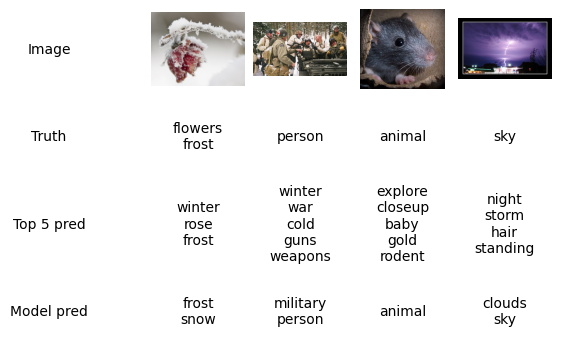
\includegraphics[width=0.9\textwidth]{PNG/test-topk}
	\caption{
	Приклад адаптивної к-сті лейблів.
	'Truth' - правдиве маркування,
	'Top 5 pred' - ілюстрація вибору top $k$, при $k=5$,
	'Model pred' - приклад роботи нашої моделі.
	}
	\label{figure:test-topk}
\end{figure}

Один із сучасних підходів як-от CNN-RNN \cite{cnn-rnn},
розглядає задачу маркування як задачу перекладу зображення в текст (image to text),
де CNN - це кодувальник (encoder), а RNN (decoder) автоматично виконує як задачу маркування,
так і задачу динамічного вибору кількості лейблів, однак є певні обмеження
накладенні на порядок класів.


\chapter{Моделювання}

На основі проведного аналізу альтернатив, дана робота пропонує розглянути
мультимодальну систему (обробляє зобарження і текст), яка складається із чотирьох компонентів (\figurename{\ref{figure:composite}})

\begin{figure}[!ht]
	\centering
	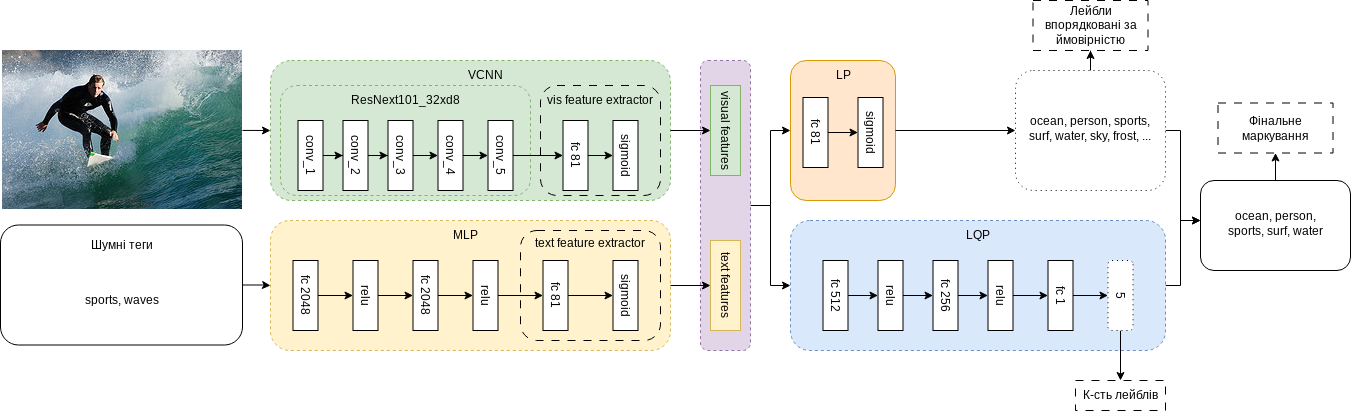
\includegraphics[width=0.9\textwidth]{PNG/composite}
	\caption{Архітектура композитної системи}
	\label{figure:composite}
\end{figure}

\section{VCNN}

Модель VCNN (\figurename{\ref{figure:composite}}) призначена для вивчення особливостей (features) із зображення.
Отримує на вхід піселі зображення $I$, у формі матриці розмірності $(B,C,W,H)$, де
$B$ - к-сть зображень у групі для тегування,
$C$ - к-сть каналів у зображеннях зазвичай 1 або 3, Grey або RGB відповідно,
$W,H$ - розмірність зображень.

За базове рішення використовуєтсья ResNext101\_32x8d \cite{resnext} (сучасна версія resnet),
із адаптованим класифікатором, натреновану на датасеті ImageNet \cite{deng2009imagenet}.

На виході даної моделі ми отримуємо вектор вірогідностей $vf$ (visual feature vector),
який вказує вірогідність маркування зображення класом $j$ на основі візуальної інформації.


\section{MLP}

MLP (\figurename{\ref{figure:composite}}) - аналізує текстові особливості (text features) тегів до зображення.
Теги до зображення $i$ репрезентуються як бінарний вектор $I = [1,0,1,0, ..., N]$,
де 1 - це наявність тегу, а $N$ - к-сть тегів.

Головна причина вибору звичайної MLP моделі для аналізу текстової інформації - це
те, що вхідна інформація - це шумні теги (наприклад: для фото кота - теги "Канада", "Кіт").

На виході даної моделі ми отримуємо вектор $tf$ вірогідностей (text feature vector),
який вказує вірогідність маркування зображення класом $j$ на основі текстової інформації.


\section{LP}

LP (\figurename{\ref{figure:composite}}) - аналізує вектор вірогідності $v$,
який є композицією векторів $vf$ та $tf$: $v = [vf, tf]$.

На виході даної моделі ми отримуємо вектор вірогідностей, який комбінує інформацію отриману як із візуальної так і з
текстової інформації.


\section{LQP}

Модель LQP (\figurename{\ref{figure:composite}}) аналізує кількість лейблів на основі вектору вірогідностей $v$,
який є композицією векторів $vf$ та $tf$: $v = [vf, tf]$.

Існує два підходи до визначення к-сті за допомогою нейронних мереж: класифікація та регресія.
LQP - регресійна модель.

Оскільки регресійні моделі досить швидко перенавчаються (overfitting), то необхідно задіяти регуляризацію.
В даній роботі, в якості регуляризатора задіяні Dropout шари \cite{dropout}, із вірогідністю відкидання (dropout rate) $0.5$.

На виході даної моделі є число, яке вказує на кількість лейблів у зображенні.


\section{Процес тренування}

Система є мультимодальною, і містить досить багато параметрів, тому тренувати її за один раз буде складно
і буде виникати проблема затухаючого градієнта.

Тому тренування відбуваєтсья у декілька стадій, у якому кожна із моделей тренується окремо
(деякі з них можна тренувати синхронно).


\paragraph{\textbf{Цільові функції}\\}

Для початку варто розглянути цільові функції (функція втрат, loss function).
Дані функції є базовим компонентом глибинного навчання.

В даній роботі використовуютсья дві функції: BCEWithLogitsLoss та MSELoss.

\paragraph{\textit{BCEWithLogitsLoss}\\}

Для тренування класифікаційних моделей (VCNN, MLP, LP) вихідні логіти $z_{ij}$
для групи (batch) зображень $I_N$ при $i = 1...N$, $j = 1...C$,
де $N$ - кількість зображень в групі, $C$ - кількість цільових класів,
цільова функція має вигляд:

\begin{equation}
\mathcal{L}_{cls} = \frac{1}{NC} \sum_{i}^{N} \sum_{j}^{C}
y_{ij} \cdot ln(\sigma(z_{ij})) + (1 - y_{ij}) \cdot ln(1 - \sigma(z_{ij}))
\end{equation}

, де $y_{ij} = 1$ якщо зображення $i$ анотоване класом $j$, інакше - $y_{ij} = 0$,
а $\sigma(\cdot)$ - це сигмоїдальна активаційна функція

\paragraph{\textit{MSELoss}\\}

Для тренування регресійної моделі LQP вихідні логіти $z_i$
для групи (batch) зображень $I_N$ при $i = 1...N$,
де $N$ - кількість зображень в групі,
цільова функція має вигляд:

\begin{equation}
\mathcal{L}_{reg} = \frac{1}{N} \sum_{i}^{N}
(y_i - z_i)^2
\end{equation}

, де $y_i$ - це кількість лейблів для зображення $I_i$.


\paragraph{\textbf{Тренування VCNN}\\}

Тренування моделі ResNext \cite{resnext} з нуля є досить складною задачою (дана модель має $\approx$ 80M параметрів),
адже для цього потрібні значні обчислювальні потужності.

Саме тому вироистовується натренована модель із адаптованим класифікатором (visual feature extractor) (\figurename{\ref{figure:composite}}), яка підганяється (finetuned) на обраному датасеті.

Існує два підходи для підгонки:

\begin{enumerate}[1)]
	\item Підгонка всієї моделі:
	всі шари моделі підганяються (дотреновуються) з низькою швидкістю навчання (learning rate).
	Даний підхід вимагає великої обчислювальної потужності, однак надає високу точність та
	досить таки швидко тренується (в порівнянні із тренуванням з нуля).

	\item Підгонка класифікатора:
	відбуваєтсья тренування тільки класифікатора, фіксуючи всі інші параметри моделі.
	Даний підхід значно пришвидшує тренування в обмін на певну деградацію точності в порівнянні із 1-им варіантом.
\end{enumerate}

В даній роботі використовується 2 варіант підгонки.


\paragraph{\textbf{Тренування MLP}\\}

Дана модель є звичайним багатошаровим персептроном, тому її тренування досить таки прямолінійне.


\paragraph{\textbf{Тренування LP}\\}

Дана модель призначена для обрахування вірогідностей на основі вектору $f = [vf, tf]$, оскільки вона
складається із одного шару то її тренування також очевидне.


\paragraph{\textbf{Тренування LQP}\\}

Дана модель є регресійною, її тренування також є очевидним, однак варто нормалізувати
вхідну к-сть лейблів, так як це пришвдшить та/або покращить збіжність моделі.


\section{Процес тестування}

\paragraph{\textbf{Тестування класифікаційних моделей (VCNN, MLP, LP)}\\}

Кожна із даних моделей обраховує вектор ймовірностей $P$,
для тестування необхідно перевести вектор ймовірностей (наприклад: $P = [0.9, 0.6, 0.1, 0.4, 0.6]$)
у вигляд маркування (наприклад: $M = [1,1,0,0,1]$).

\paragraph{Розглянемо два основних підходи:}

\begin{enumerate}[1)]
	\item Порогове значення (threshold):
	для вектору ймовірностей $P$ та порогу $T$ - вектор маркувань обраховується наступним чином:
	якщо $y_i > T$, то маркуємо $1$, інакше $0$.
	Наприклад при $T = 0.5$: $[0.9, 0.6, 0.1, 0.4, 0.6] \to [1,1,0,0,1]$.

	\item Найкращі $k$ (top $k$):
	для вектору ймовірностей $P$ та числа $k$ - вектор маркувань обраховується наступним чином:
	маркуємо $1$ найкращі $k$ ймовірностей, інакше $0$.
	Наприклад при $k = 4$: $[0.9, 0.6, 0.1, 0.4, 0.6] \to [1,1,0,1,1]$.
\end{enumerate}

Оскільки дані моделі \textbf{не передбачають} передбачення кількості лейблів,
то для тренування даних моделей використовується метод top $k$, при чому
$k$ обирається на основі правдивого маркування.

Тобто для зображення $I$,
із маркуванням $Y = [1,0,0,1,1]$,
і вектором ймовірностей $P = [0.8,0.9,0.1,0.3,0.2]$
та результуючим вектором маркувань $M$:
$k = 3$, так як $Y$ містить 3 промаркованих класи,
перетворення $P \to M \equiv [0.8,0.9,0.1,0.3,0.2] \to [1,1,0,1,0]$


\paragraph{\textbf{Тестування композитної моделі}\\}

Для тестування композитної моделі (\figurename{\ref{figure:composite}})
необхідно обрахувати результуючі значення для моделей LP та LQP, і обрати
top $k$ лейблів LP, де $k$ - це передбачення LQP.


\chapter{Експерименти}

\section{Датасет}

Один із найбіль часто використовуваних датасетів для тестування моделей анотації зображень - NUS-WIDE \cite{nus-wide-civr09},
він складаєтсья із 269,655 зображень, 81 лейблу, та $\approx$ 5000 тегів в якості сторонньої текстової інформації.
Для проведення тренування/тестування використовується розподіл, надведений разом із
датасетом, так як він є збалансовний настільки, наскільки це можливо (\figurename{\ref{figure:nus-wide-dist}}).

\begin{figure}[!ht]
	\centering
	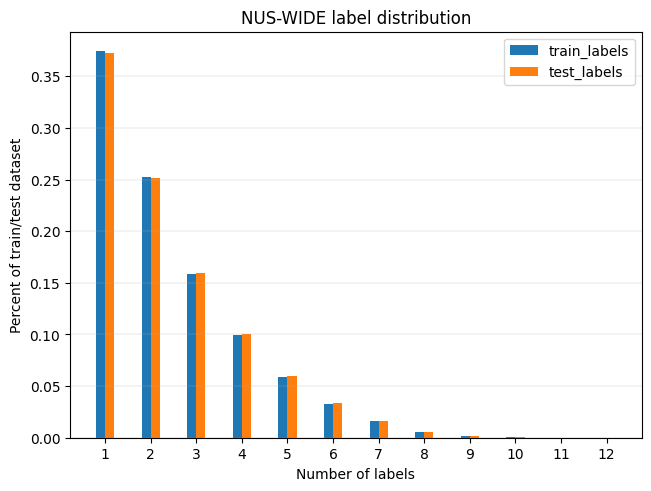
\includegraphics[width=0.9\textwidth]{PNG/nus-wide-dist}
	\caption{Розподіл лейблів у тренувальному/тестовому датасеті}
	\label{figure:nus-wide-dist}
\end{figure}

Важливо відмітити, що даний датасет містить посиланя на зображення на ресурсі Flickr, і деякої частина цих
зображень вже там немає. Також буде використано тільки 1000 найбільш частих тегів з $\approx$ 5000,
при чому зображення, які не містять жодного тега відфільтровано.

Далі наведено деякі числові характеристики тренувальної/тестової вибірок:

\begin{center}
\begin{tabular}{ccc}
		\toprule[2pt]
           & Тренування & Тестування \\
        \midrule
        Кількість зобаржень & 121962  & 81636 \\
        Середня к-сть лейблів & 2.42  & 2.43 \\
        Медіана к-сть лейблів & 2  & 2 \\
        Мінімальна к-сть лейблів & 1  & 1 \\
        Максимальна к-сть лейблів & 12  & 13 \\
        \bottomrule[2pt]
\end{tabular}
\captionof{table}{Характеристики тренувальної/тестової вибірок}
\end{center}

\clearpage


\section{Метрики}

Для оцінки точності будуть використовуватись метрики, які є загально вживаними для оцінки
задачі анотації зображень (multi-label image annotation).

\begin{equation}
\begin{aligned}
P_C &= \frac{1}{C} \sum_{j=1}^C \frac{NI^c_j}{NI^p_j} & P_I &= \frac{\Sigma^N_{i=1} NL^c_i}{\Sigma^N_{i=1} NL^p_i} \\
R_C &= \frac{1}{C} \sum_{j=1}^C \frac{NI^c_j}{NI^g_j} & R_I &= \frac{\Sigma^N_{i=1} NL^c_i}{\Sigma^N_{i=1} NL^g_i} \\
F1_C &= \frac{2 \cdot P_C \cdot R_C}{P_C + R_C} & F1_I &= \frac{2 \cdot P_I \cdot R_I}{P_I + R_I} \\
\end{aligned}
\end{equation}

,де \begin{itemize}[*]
        \item $C$ - к-сть класів
        \item $N$ - к-сть тестових зображень
        \item $NI^c_j$ - к-сть зображень які \textbf{коректно} промарковано як клас $j$
        \item $NI^g_j$ - к-сть зображень які мають клас $j$
        \item $NI^p_j$ - к-сть зображень які промарковано як клас $j$
        \item $NL^c_i$ - к-сть \textbf{коректно} промаркованих лейблів для зображення $i$
        \item $NL^g_i$ - к-сть лейблів які має зображення $i$
        \item $NL^p_i$ - к-сть промаркованих лейблів для зображення $i$
\end{itemize}

Варто відзначити, що дані метрики є зміщеними (biased),
при чому по-класові метрики ($C$) зміщені в сторону рідкісних класів,
а загальні метрики ($I$) - в сторону частих класів.

\clearpage

Для того що отримати унфіормене представлення про ефективність моделі
буде використовуватись наступна метрика,
яка бере до уваги як $F1_C$ так і $F1_I$, що полегшує інтерпретацію результатів:

\begin{equation}
F1_H = \frac{2 \cdot F1_C \cdot F1_I}{F1_C F1_I}
\end{equation}


\clearpage


\section{Тренування}

Для програмної реалізації запропонованої моделі було використано PyTorch.

Оскільки в даній роботі, використовується модель ResNext \cite{resnext} натренована
на датасеті ImageNet \cite{deng2009imagenet}, то для вхідних зображень потрібно
застосувати певне перетворення:

\begin{enumerate}[1)]
	\item Зміна розміру (Resize) $232 \times 232$,
	використовуючи білінійну інтерполяцію
	\item Центральний кроп (Central crop) $224 \times 224$
	\item Зміна масшатбу (Rescale) [0,1]
	\item Нормалізація на основі статистичних величин ImageNet \cite{deng2009imagenet}.
	А саме: mean = [0.485, 0.456, 0.406] та std = [0.229, 0.224, 0.225]
\end{enumerate}

Дане перетворення доступно у біблоітеці PyTorch.


\paragraph{\textbf{Параметри навчання}\\}

Класифікаційні моделі VCNN та MLP навчались із
швидкістю навання (learning rate) 0.001, а LP - зі швидкістю 0.01.
Також для начання цих трьох моделей використовувався контроллер швикдості навчання
(learning rate scheduler), який множив швидкість навчання на 0.5, досягаючи
5-ої та 10-ої епохи.

Регресійна модель LQP навчалась із сталою швидкістю навчання (learning rate) 0.0005.

Для всіх навчання всіх вище згаданих моделей використовувався оптимізатор
AdamW, із параметром l1 регуляризації (weight decay) 0.0003.

Розмір групи (batch size) 32.

Також варто відзначити, що в даній роботі епоха - це 10\% від усіх даних,
при чому після кожної епохи дані перемішуються (shuffle), отримаючи
нові 10\% даних.


\paragraph{\textbf{Процес навчання}\\}

Оскільки дана робота розглядає базове тренування всіх компонентів моделі,
то варто розглянути саме процес тренування, для того щоб вказати місця, які
потенційно можна покращити для збільшення точності моделі.

\begin{figure}[h]
\centering
	\subcaptionbox{Навчання VCNN}
		{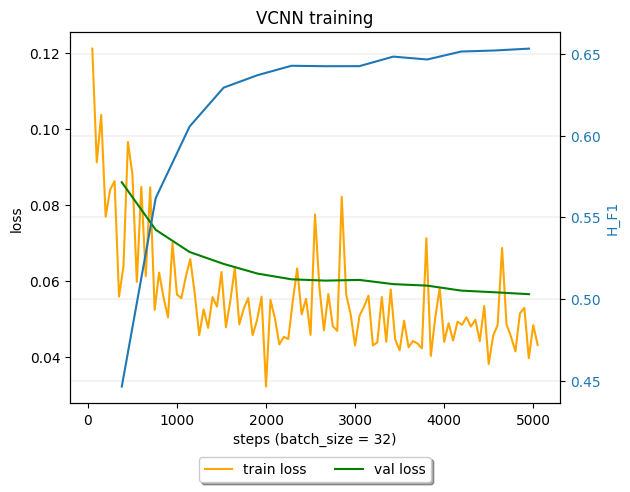
\includegraphics[width=0.45\linewidth]{PNG/vcnn-train}}
	\subcaptionbox{Навчання MLP}
		{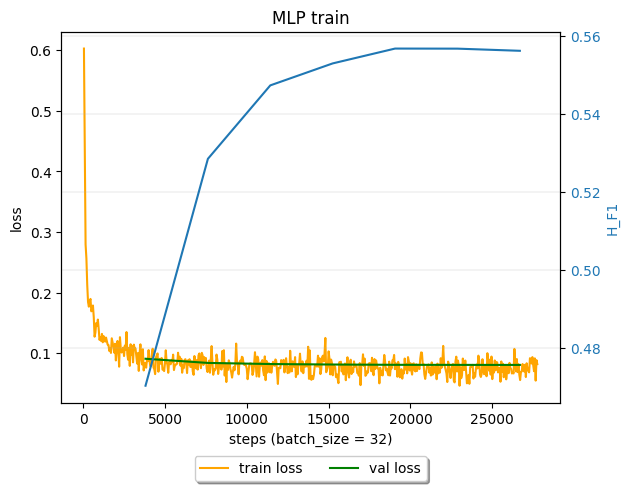
\includegraphics[width=0.45\linewidth]{PNG/mlp-train}}
	\subcaptionbox{Навчання LP}
		{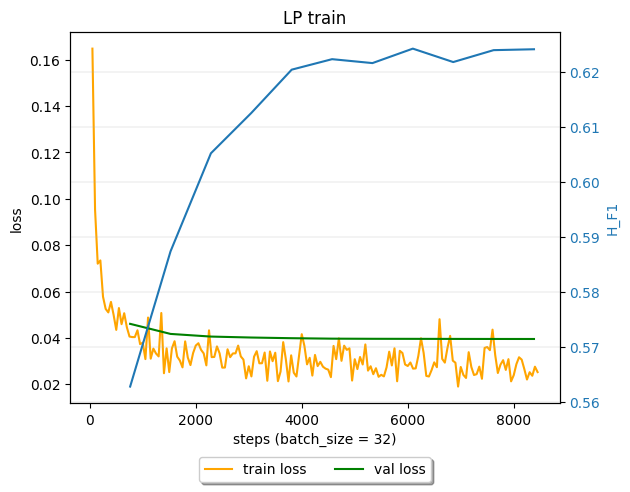
\includegraphics[width=0.45\linewidth]{PNG/lp-train}}
	\subcaptionbox{Навчання LQP}
		{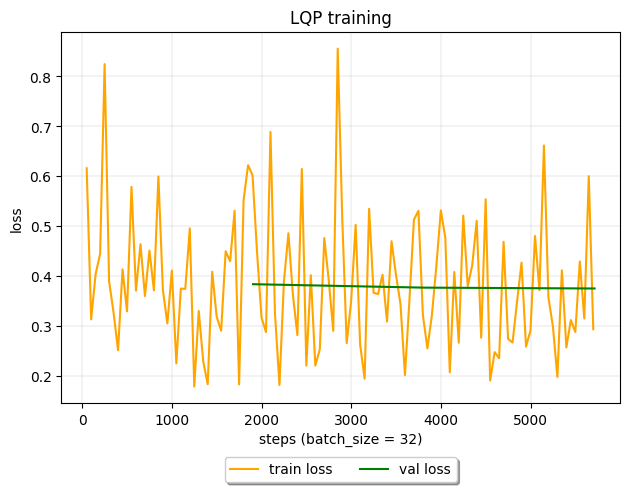
\includegraphics[width=0.45\linewidth]{PNG/lqp-train}}
\caption{Процес навчання моделей}
\end{figure}


% створюємо Висновки
\conclusions

\printbibliography

\append{Код лістинг}

\end{document}
